\documentclass[11pt]{article}
\usepackage[a4paper,margin=1in]{geometry}
\reversemarginpar
\usepackage{mathtools, amsthm, amssymb, amsmath}
\usepackage{multicol}
\usepackage{todonotes}

\usepackage{subcaption}
\usepackage{longtable}

\usepackage[style=numeric, sorting=none]{biblatex}
\addbibresource{MV.bib}

\usepackage{graphicx}
\graphicspath{{./picture/}}

\usepackage{subcaption}

\usepackage{tikz}
\usetikzlibrary{positioning}

\usepackage{rotating}

\newtheorem{theorem}{Theorem}[section]
\theoremstyle{definition}
\newtheorem{definition}[theorem]{Definition}
\newtheorem{example}[theorem]{Example}

\DeclareMathOperator{\dom}{dom}

\title{Generating of Music Variations: Dynamical Systems Approach}
\author{Rajamangala University of Technology Thanyaburi\\Kanatsanun Sub-udom\\Wannasa Rianthong\\Patipan Somwong}

\begin{document}

\section{Literature Review}

\begin{definition}
Let $\mathbb{N}_n$ denote the sequence of natural number with $n$-elements defined by:
\[ \mathbb{N}_n = \{ 1, 2, \dots, n \}  \]
\end{definition}

\subsection{Fourth-Order Runge–Kutta Method}
While analytical solutions exist for some differential equations, many require numerical approaches to approximate their behavior. The field of mathematics offers a numerical methods for solving both single and systems of linear and nonlinear differential equations. Popular examples include the Euler method and Taylor series methods. However, when it comes to achieving a balance between accuracy and efficiency, the Runge-Kutta method reigns supreme for approximating solutions.

The Runge-Kutta method \cite{bose_numerical_2019} is a numerical methods for approximating solutions to ordinary differential equations. These equations describe how a quantity changes with respect to another variable, but often cannot be solved exactly. The Runge-Kutta method tackles these problems by breaking down the interval of interest into smaller subintervals and iteratively calculating the solution at each subinterval. 

Let $\dot{y} = f(t,y)$. The approximation of $y_{i+1}$ by fourth-order Runge–Kutta method is given by:
\begin{align*}
y_{i+1} &= y_i + \dfrac{h}{6}(k_1 + 2k_2 + 2k_3 + k_4), \\
k_1 &= f(t_i, y_i), \\
k_2 &= f\left( t_i + \dfrac{h}{2}, y_i + \dfrac{h}{2}k_1 \right), \\
k_3 &= f\left( t_i + \dfrac{h}{2}, y_i + \dfrac{h}{2}k_2 \right), \\
k_4 &= f(t_i + h, y_i + hk_3),
\end{align*}
\label{fig:RK4}
where $i = 0,1,2,...$ and $h$ is the step size, $y$ is the variable and $t$ is time.

\section{Main Result}
This section explores the musical variations from a chaotic mapping method and combining musical variations from a chaotic mapping and melodic variation with expanded rhythm methd. We will demonstrate this method through two examples. In the first example, we will illustrate how a chaotic map can be used to generate variations in musical pitch. In the second example, we will combine this method with another method for expanding rhythm to create more interesting musical variations.

\subsection{Musical Variations from a Chaotic Mapping}

For a musical sheet, let $m$ be a positive integer representing a number of notes, $P = \{p_0, p_1, \dots, p_{m-1}\}$ be a sequence of music pitches and  
\begin{equation} \label{eq: odes}
\dot{x}(t) = f(t,x)
\end{equation}
be a chaotic dynamical system with an initial condition $x(0) \in \mathbb{R}^n$, where $x(t) = \left(x_1(t), \ldots, x_n(t)\right)$ is differntiable for all $t \geq 0$.
Let $f: \mathbb{R}_{+} \times \mathbb{R}^n \to \mathbb{R}^n$ is a continuous function. 
Given a sequece
$ V = \displaystyle\left\{\phi_i(kh) \right\}_{k=0}^{m-1}$ 
for some $i \in \mathbb{N}_n$, where $\phi_i$ is a numerical solution in $i$-th component to \eqref{eq: odes} with a step size of $h$.
Let $ f: V \to P$ be a mapping defined by 
$f(v_k) = f(\phi_i(kh)) := p_k$ for all $k \in \{0\}\cup\mathbb{N}_{m-1}$.

Consequently, we introduce another sequence $\widetilde{V}_i = \left\{\tilde{\phi}_i(kh) \right\}_{k=0}^{m-1}$, where $\tilde{\phi}_i$ is a numerical solution with a new initial condition $\tilde{x}(0) \in \mathbb{R}^n$ $i$-th component to \eqref{eq: odes}, 
when $\tilde{x}(0)$ start not far from $x(0)$, i.e., $ \left\lVert x(0) - \tilde{x}(0) \right\rVert \leq d$ for some small positve number $d \in \mathbb{R}$. Then, we define another mapping $g: \widetilde{V} \to P$ by: 
\[ g(\tilde{v}_k) = g\left(\tilde{\phi}_i(kh)\right) := 
\begin{cases}
  f(\phi_i(b)) & \text{ if }\exists a, b \in \dom{\phi_i} \text{ s.t. } \phi_i(a) < \tilde{\phi}(kh) \leq \phi_i(b) \\
  f(\phi_i(a)) & \text{ if } \tilde{\phi}(kh) < \phi_i(a) \text{ for all } a \in \dom{\phi_i} \\
  f(\phi_i(b)) & \text{ otherwise} .
\end{cases}
\]
This procedure yields, a new sequence of music pitches $\widetilde{P} =\{ \tilde{p}_1, \tilde{p}_2, \dots, \tilde{p}_n \}$.

\begin{example}
Let a sequence of pitches of 12 variations on Ah vous dirai-je Maman in the first 3 bars in Figure \ref{fig:Dabby1} denoted by $P = \{C4, C4, G4, G4, A4, A4, G4, F4, F4, E4, E4 \}$ in Figure \ref{subfig:mp} and Lorenz system be a dynamical system with chaotic behavior by giving Lorenz parameters $r = 28, \sigma=10$ and $b = 2.6667 $. Then the numerical solution of Lorenz system using fourth-order Runge–Kutta method with initial condition of $(1,1,1)$ is denoted by $X = \{1.00, 1.29, 2.13, 3.74, 6.54, 11.04, 16.69, 19.56, 15.37, 7.55, 1.20\}$ in Figure \ref{subfig:traj1}, when $X$ is a sequence of x-value from numerical solution of Lorenz system. Then, a mapping from music pitch to real value denoted by $f$ result in Figure \ref{subfig:traj1mp} as follows:

\begin{center}
\begin{tabular}{|c||c|c|c|c|c|c|}
\hline
$f(x_i)$ & $f(1.00)$ & $f(1.29)$ & $f(2.13)$ & $f(3.74)$ & $f(6.54)$ & $f(11.04)$ \\
\hline
$p_i$ & C4 & C4 & G4 & G4 & A4 & A4 \\
\hline
$f(x_i)$ & $f(16.69)$ & $f(19.56)$ & $f(15.37)$ & $f(7.55)$ & $f(1.20)$ & \\
\hline
$p_i$ & G4 & F4 & F4 & E4 & E4 &  \\
\hline
\end{tabular}
\end{center}

Next, We generating a new trajectory with an initial condition of $(1.01,1,1)$ and $X^\prime = \{ 1.01, 1.30, 2.15, 3.76, 6.58, 11.10, 16.73, 19.55, 15.30, 7.48, 1.15 \} $ is a sequence of x-value from new trajectory in Figure \ref{subfig:traj2}. Then, a mapping from real value to music pitch denoted by $g$ result in Figure \ref{subfig:traj2nmp} as follows:

\begin{center}
\begin{tabular}{|c||c|c|c|c|c|c|}
\hline
$g(x^\prime_i)$ & $g(1.01)$ & $g(1.30)$ & $g(2.15)$ & $g(3.76)$ & $g(6.58)$ & $g(11.10)$ \\
\hline
$p_i$ & E4 & G4 & G4 & A4 & E4 & F4 \\
\hline
$g(x^\prime_i)$ & $g(16.73)$ & $g(19.55)$ & $g(15.30)$ & $g(7.48)$ & $g(1.15)$ & \\
\hline
$p_i$ & F4 & F4 & F4 & E4 & E4 &  \\
\hline
\end{tabular}
\end{center}
This procedure yields, as shown in Figure \ref{fig:dabby method}, a new sequence of music pitches \\ $\hat{P} =\{E4, G4, G4, A4, E4, F4, F4, F4, F4, E4, E4 \}$ in Figure \ref{subfig:nmp}. Which can be converted to sheet music in Figure \ref{fig:Dabby2}. Since this method uses the same note duration and musical notes to create a new variation, so the resulting changes in the sequence compared to the original sequence might seem relatively small.
\end{example}

\begin{figure}
\centering
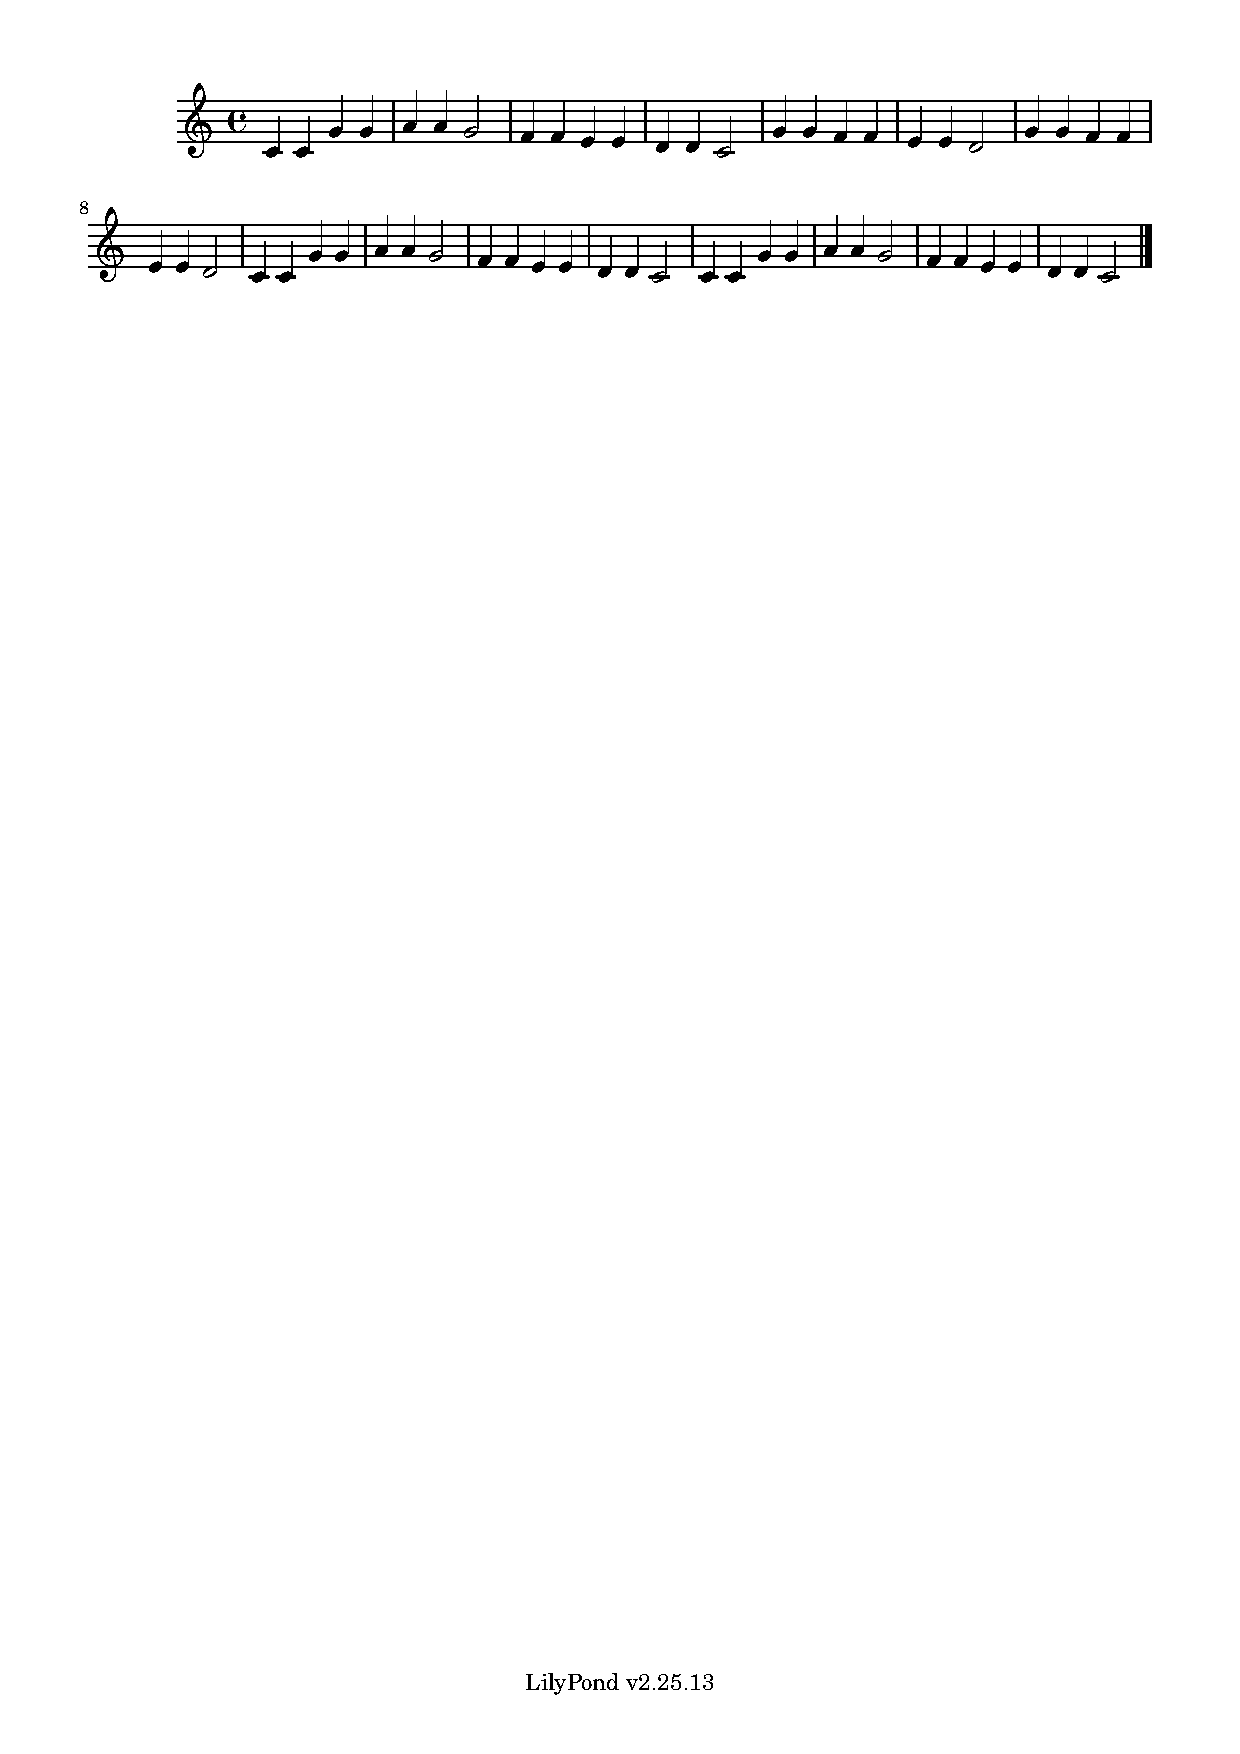
\includegraphics[trim=1cm 26.5cm 10.055cm 0.02cm, clip, scale=1]{dabby_1.pdf} % trim={left bottom right top}
\caption{The original of 12 variations on Ah vous dirai-je Maman in the first 3 bars.}
\label{fig:Dabby1} 
\end{figure}

\begin{figure}
\centering
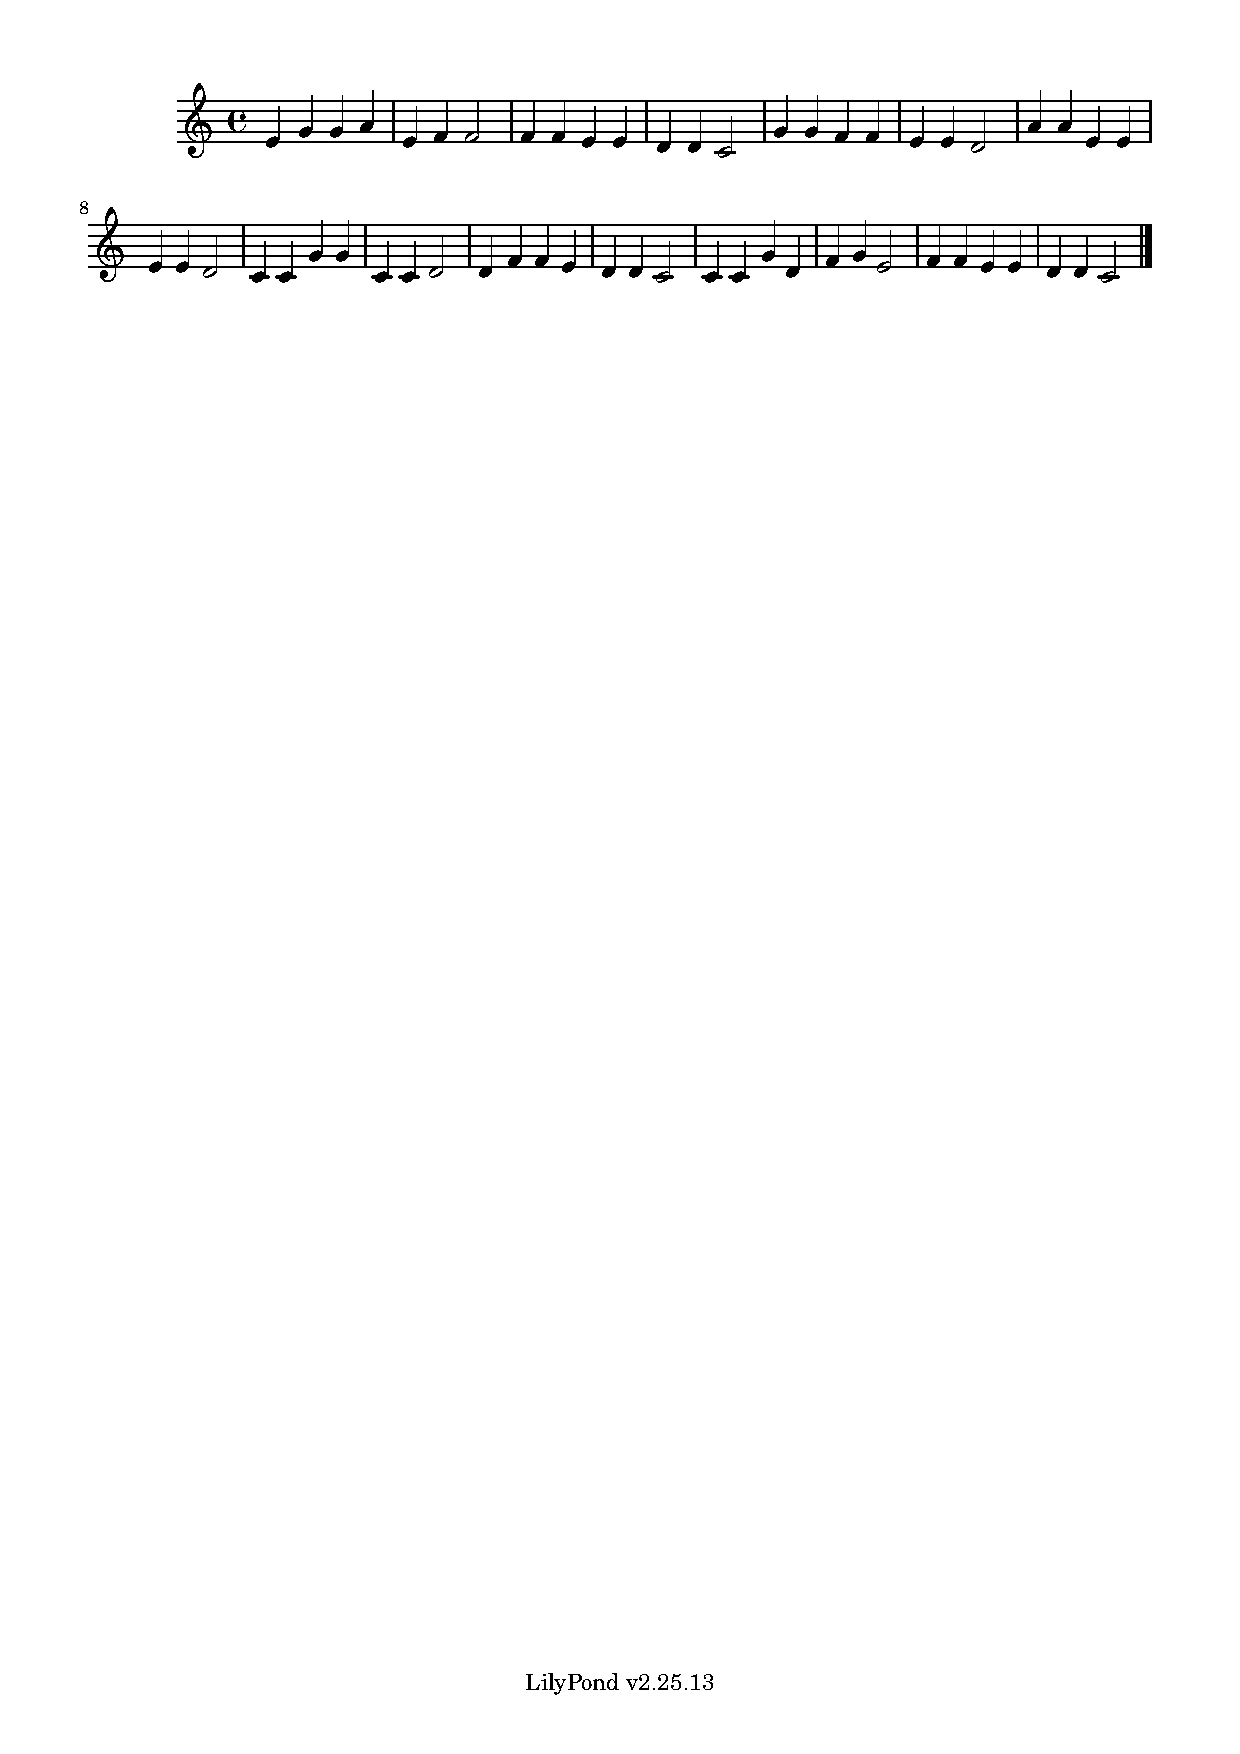
\includegraphics[trim=1cm 26.5cm 10.1cm 0.02cm, clip, scale=1]{dabby_2.pdf}
\caption{The new variation of 12 variations on Ah vous dirai-je Maman in the first 3 bars, generated by the Initial Condition $(1.01, 1, 1)$.}
\label{fig:Dabby2}
\end{figure}

\begin{figure}
\centering

\begin{subfigure}{\textwidth}
  \centering
  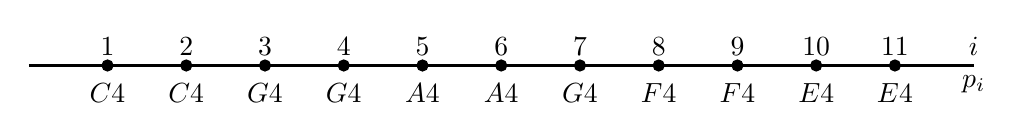
\begin{tikzpicture}
    % Draw number line
    \draw[-, thick] (0,0) -- (12,0) node[below] {$p_i$}  node[above] {$i$};

    % Data
    \foreach \i/\x/\p in {1/C4/1, 2/C4/2, 3/G4/3, 4/G4/4, 5/A4/5, 6/A4/6, 7/G4/7, 8/F4/8, 9/F4/9, 10/E4/10, 11/E4/11} {
      % Draw points and labels
      \filldraw (\i,0) circle (2pt) node[above] {$\p$};
      
      % Draw number scale below the line
      \draw (\i,-0.1) node[below] {$\x$};
    }

	\end{tikzpicture}
  \caption{The first 11 pitches of the 12 variations on Ah vous dirai-je Maman are marked below the pitch axis.}
  \label{subfig:mp}
\end{subfigure}

\vspace{5pt}

\begin{subfigure}{\textwidth}
  \centering
  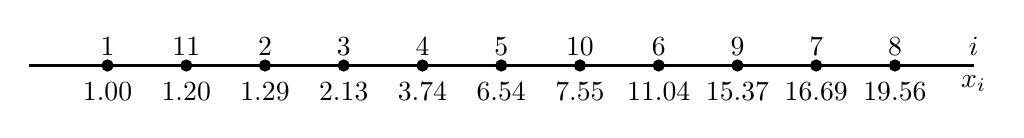
\begin{tikzpicture}
    % Draw number line
    \draw[-, thick] (0,0) -- (12,0) node[below] {$x_{i}$}  node[above] {$i$};

    % Data
    \foreach \i/\x/\p in {1/1.00/1, 2/1.20/11, 3/1.29/2, 4/2.13/3, 5/3.74/4, 6/6.54/5, 7/7.55/10, 8/11.04/6, 9/15.37/9, 10/16.69/7, 11/19.56/8} {
      % Draw points and labels
      \filldraw (\i,0) circle (2pt) node[above] {$\p$};
      
      % Draw number scale below the line
      \draw (\i,-0.1) node[below] {$\x$};
    }

  \end{tikzpicture}
  \caption{The first 11 x-components of the numerical solution of Lorenz system with initial condition of $(1,1,1)$ are marked below the x axis.}
  \label{subfig:traj1}
\end{subfigure}

\vspace{5pt}

\begin{subfigure}{\textwidth}
  \centering
  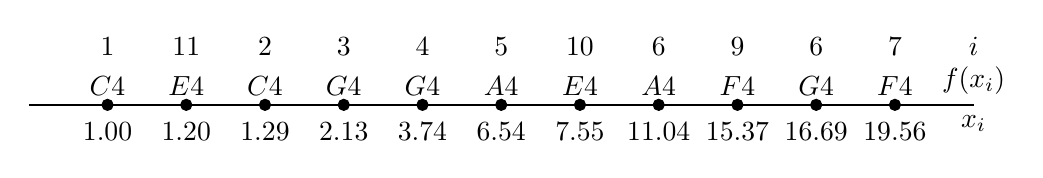
\begin{tikzpicture}
    % Draw number line
    \draw[-, thick] (0,0) -- (12,0) node[below] {$x_{i}$}  node[above] {$f(x_i)$} node[above=0.5cm] {$i$};

    % Data
    \foreach \i/\x/\p in {1/1.00/C4, 2/1.20/E4, 3/1.29/C4, 4/2.13/G4, 5/3.74/G4, 6/6.54/A4, 7/7.55/E4, 8/11.04/A4, 9/15.37/F4, 10/16.69/G4, 11/19.56/F4} {
      % Draw points and labels
      \filldraw (\i,0) circle (2pt) node[above] {$\p$};
      
      % Draw number scale below the line
      \draw (\i,-0.1) node[below] {$\x$};
    }
    
    % Display the sequence at each point
    \foreach \i/\x in {1/1, 2/11, 3/2, 4/3, 5/4, 6/5, 7/10, 8/6, 9/9, 10/6, 11/7} {
      \draw (\i,0.5) node[above] {\x};
    }
  \end{tikzpicture}
  \caption{For each x-component $x_i$, apply the $f(x_{i})$ mapping.}
  \label{subfig:traj1mp}

\end{subfigure}

\vspace{5pt}

\begin{subfigure}{\textwidth}
  \centering
  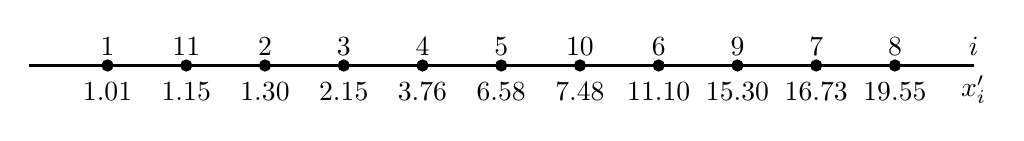
\begin{tikzpicture}
    % Draw number line
    \draw[-, thick] (0,0) -- (12,0) node[below] {$x^\prime_i$}  node[above] {$i$};

    % Data
    \foreach \i/\x/\p in {1/1.01/1, 2/1.15/11, 3/1.30/2, 4/2.15/3, 5/3.76/4, 6/6.58/5, 7/7.48/10, 8/11.10/6, 9/15.30/9, 10/16.73/7, 11/19.55/8} {
      % Draw points and labels
      \filldraw (\i,0) circle (2pt) node[above] {$\p$};
      
      % Draw number scale below the line
      \draw (\i,-0.1) node[below] {$\x$};
    }

	\end{tikzpicture}
  \caption{The first 11 x-components of the numerical solution of Lorenz system with new initial condition of $(1.01,1,1)$ are marked below the x axis.}
  \label{subfig:traj2}

\end{subfigure}

\vspace{5pt}

\begin{subfigure}{\textwidth}
  \centering
  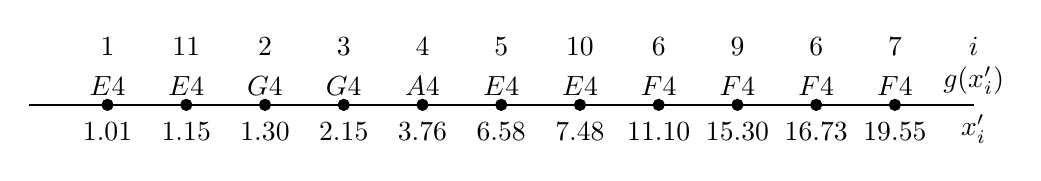
\begin{tikzpicture}
    % Draw number line
    \draw[-, thick] (0,0) -- (12,0) node[below] {$x^\prime_{i}$}  node[above] {$g(x^\prime_{i})$} node[above=0.5cm] {$i$};

    % Data
    \foreach \i/\x/\p in {1/1.01/E4, 2/1.15/E4, 3/1.30/G4, 4/2.15/G4, 5/3.76/A4, 6/6.58/E4, 7/7.48/E4, 8/11.10/F4, 9/15.30/F4, 10/16.73/F4, 11/19.55/F4} {
      % Draw points and labels
      \filldraw (\i,0) circle (2pt) node[above] {$\p$};
      
      % Draw number scale below the line
      \draw (\i,-0.1) node[below] {$\x$};
    }
    
    % Display the sequence at each point
    \foreach \i/\x in {1/1, 2/11, 3/2, 4/3, 5/4, 6/5, 7/10, 8/6, 9/9, 10/6, 11/7} {
      \draw (\i,0.5) node[above] {\x};
    }
  \end{tikzpicture}
  \caption{For each x-component $x^\prime_i$, apply the $g(x^\prime_{i})$ mapping.}
  \label{subfig:traj2nmp}

\end{subfigure}

\vspace{5pt}

\begin{subfigure}{\textwidth}
  \centering
  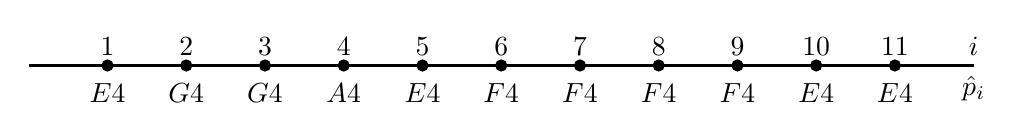
\begin{tikzpicture}
    % Draw number line
    \draw[-, thick] (0,0) -- (12,0) node[below] {$\hat{p}_i$}  node[above] {$i$};

    % Data
    \foreach \i/\x/\p in {1/E4/1, 2/G4/2, 3/G4/3, 4/A4/4, 5/E4/5, 6/F4/6, 7/F4/7, 8/F4/8, 9/F4/9, 10/E4/10, 11/E4/11} {
      % Draw points and labels
      \filldraw (\i,0) circle (2pt) node[above] {$\p$};
      
      % Draw number scale below the line
      \draw (\i,-0.1) node[below] {$\x$};
    }

	\end{tikzpicture}
  \caption{The new variation of the first 11 pitches  are marked below the pitch axis.}
  \label{subfig:nmp}

\end{subfigure}

\caption{The visualizes how a chaotic mapping method can be used to generate musical variations}
\label{fig:dabby method}
\end{figure}

\subsection{Melodic Variation with Expanded Rhythm Method} 
Given a note duration denoted by $\phi$ and divided into $D$ equal parts, the duration, $R$, of each individual division is defined by the following equation:
$$ R = \frac{\phi}{D}.  $$
\textbf{Note:} In musical theory, equal parts refers to divisions that all have the same duration.

\begin{example}
Consider the music piece 12 variations on Ah vous dirai-je Maman, illustrated in Figure \ref{fig:MV1}. The Figure shows that we already have 6 quarter notes and 1 half note.

If we want to divide each musical note into 4 parts, we can find the duration of each individual division as follows:
\begin{enumerate}
  \item[$\bullet$] Half note to 4 parts: $$R = \frac{\phi}{D} = \frac{2}{4} = 0.5$$
  \item[$\bullet$] Quarter note to 4 parts: $$R = \frac{\phi}{D} = \frac{1}{4} = 0.25$$
\end{enumerate}

Following this calculation, a half note can be divided into 4 eighth notes, and a quarter note can be divided into 4 sixteenth notes. This division is represented by the sequence \\ $P = \{C4, C4, C4, C4, C4, C4, C4, C4, G4, G4, G4, G4, G4, G4, G4, G4, A4, A4, A4, A4, A4, A4, \\ A4, A4, G4, G4, G4, G4 \}$ which can be converted to sheet music, as shown in Figure \ref{fig:MV2}.
\end{example}

\begin{figure}
\centering
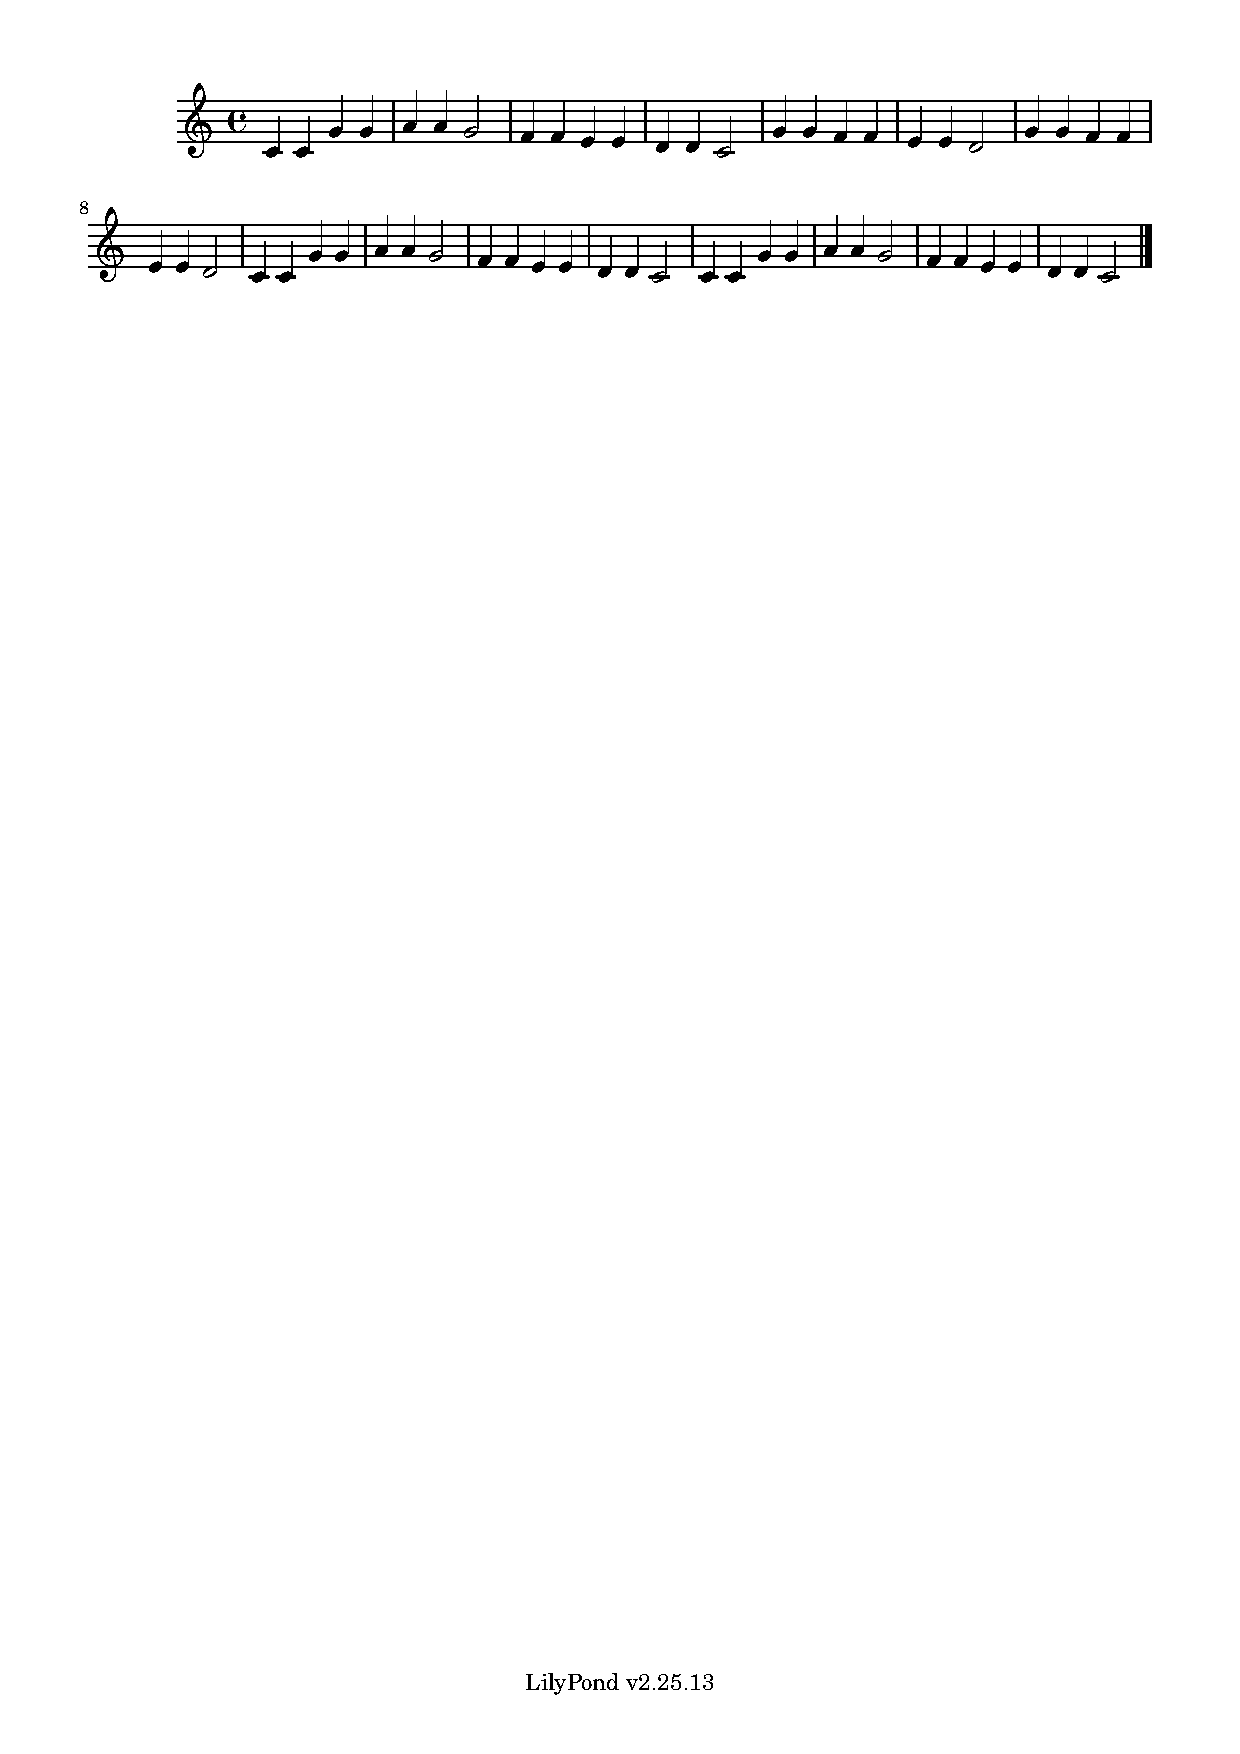
\includegraphics[trim=1cm 26.5cm 12.35cm 0.02cm, clip, scale=1]{dabby_1.pdf}
\caption{The original of 12 variations on Ah vous dirai-je Maman in the first 2 bars.}
\label{fig:MV1} 
\end{figure}

\begin{figure}
\centering
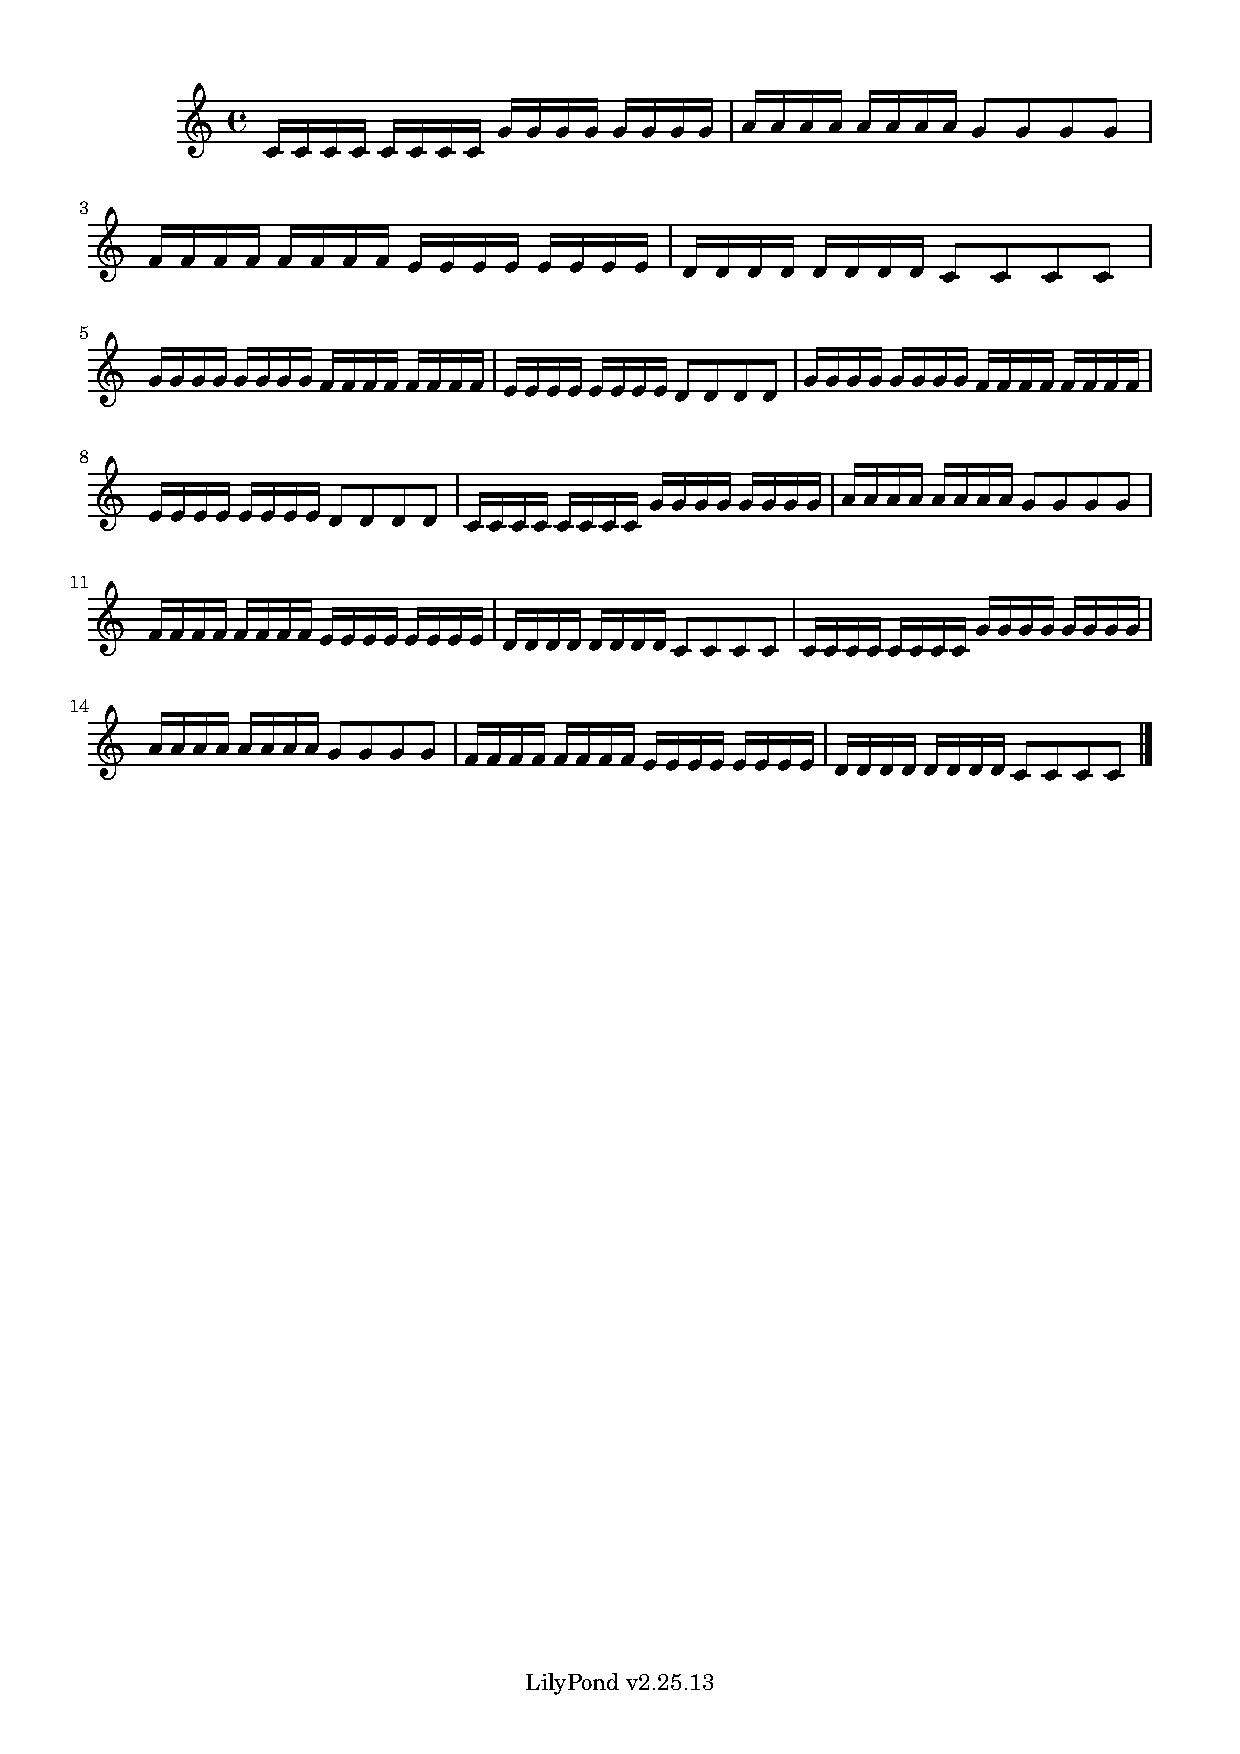
\includegraphics[trim=1cm 26.5cm 1cm 0.5cm, clip, scale=0.6]{melody_variation.pdf}
\caption{The melodic variation of Ah vous dirai-je, maman in the first 2 bars.}
\label{fig:MV2}
\end{figure}

\subsection{Combining Musical Variations from a Chaotic Mapping and Melodic Variation with Expanded Rhythm}

For a musical sheet, let $m$ be a positive integer representing a number of notes, $P = \{p_0, p_1, \dots, p_{m-1}\}$ be a sequence of music pitches and  
\begin{equation} \label{eq2: odes}
\dot{x}(t) = f(t,x)
\end{equation}
be a chaotic dynamical system with an initial condition $x(0) \in \mathbb{R}^n$, where $x(t) = \left(x_1(t), \ldots, x_n(t)\right)$ is differntiable for all $t \geq 0$.
Next, let $q$ be a positive integer representing a number of expanded notes, $P^\prime = \{p^\prime_0, p^\prime_1, \dots, p^\prime_{q-1}\}$ be a sequence of expanded music pitches and $f: \mathbb{R}_{+} \times \mathbb{R}^n \to \mathbb{R}^n$ is a continuous function. 
Given a sequece
$ V = \displaystyle\left\{\phi_i(kh) \right\}_{k=0}^{m-1}$ 
for some $i \in \mathbb{N}_n$, where $\phi_i$ is a numerical solution in $i$-th component to \eqref{eq2: odes} with a step size of $h$.
Let $ f: V \to P$ be a mapping defined by 
$f(v_k) = f(\phi_i(kh)) := p_k$ for all $k \in \{0\}\cup\mathbb{N}_{m-1}$.

Consequently, we introduce another sequence $\widetilde{V}_i = \left\{\tilde{\phi}_i(kh) \right\}_{k=0}^{q-1}$, where $\tilde{\phi}_i$ is a numerical solution with a new initial condition $\tilde{x}(0) \in \mathbb{R}^n$ $i$-th component to \eqref{eq2: odes}, 
when $\tilde{x}(0)$ start not far from $x(0)$, i.e., $ \left\lVert x(0) - \tilde{x}(0) \right\rVert \leq d$ for some small positve number $d \in \mathbb{R}$. Then, we define another mapping $g: \widetilde{V} \to P$ by: 
\[ g(\tilde{v}_k) = g\left(\tilde{\phi}_i(kh)\right) := 
\begin{cases}
  f(\phi_i(b)) & \text{ if }\exists a, b \in \dom{\phi_i} \text{ s.t. } \phi_i(a) < \tilde{\phi}(kh) \leq \phi_i(b) \\
  f(\phi_i(a)) & \text{ if } \tilde{\phi}(kh) < \phi_i(a) \text{ for all } a \in \dom{\phi_i} \\
  f(\phi_i(b)) & \text{ otherwise} .
\end{cases}
\]
This procedure yields, a new sequence of music pitches $\widetilde{P} =\{ \tilde{p}_1, \tilde{p}_2, \dots, \tilde{p}_q \}$.

\begin{example}
Let a sequence of pitches of 12 variations on Ah vous dirai-je Maman in the first 4 bars in Figure \ref{fig:DabbyER1} denoted by $P = \{C4, C4, G4, G4, A4, A4, G4, F4, F4, E4, E4, D4, D4, C4 \}$ in Figure \ref{subfig2:mp} and Lorenz system be a dynamical system with chaotic behavior by giving Lorenz parameters $r = 28, \sigma=10$ and $b = 2.6667 $. If we consider the first bar of 12 variations on Ah vous dirai-je Maman by melodic variation with expanded rhythm, $P^\prime = \{C4, C4, C4, C4, C4, C4, C4, \\ C4, G4, G4, G4, G4, G4, G4, G4, G4 \}$ will be a sequence of expanded music pitches.
Then the numerical solution of Lorenz system using fourth-order Runge–Kutta method with initial condition of $(0.5,0.5,0.5)$ is denoted by $X = \{0.50, 0.65, 1.08, 1.91, 3.41, 6.03, 10.33, 16.04, 19.69, 16.35, 8.51, \\ 1.74, -2.45, -4.80\}$ in Figure \ref{subfig2:traj1}, when $X$ is a sequence of x-value from numerical solution of Lorenz system. Then, a mapping from music pitch to real value denoted by $f$ result in Figure \ref{subfig2:traj1mp} as follows:

\begin{center}
\begin{tabular}{|c||c|c|c|c|c|c|c|}
\hline
$f(x_i)$ & $f(0.50)$ & $f(0.65)$ & $f(1.08)$ & $f(1.91)$ & $f(3.41)$ & $f(6.03)$ & $f(10.33)$ \\
\hline
$p_i$ & C4 & C4 & G4 & G4 & A4 & A4 & G4 \\
\hline
$f(x_i)$ & $f(16.04)$ & $f(19.69)$ & $f(16.35)$ & $f(8.51)$ & $f(1.74)$ & $f(-2.45)$ & $f(-4.80)$ \\
\hline
$p_i$  & F4 & F4 & E4 & E4 & D4 & D4 & C4  \\
\hline
\end{tabular}
\end{center}

Next, We generating a new trajectory with an initial condition of $(0.6,0.5,0.5)$ and $X^\prime = \{ 0.60, 0.73, 1.21, 2.13, 3.79, 6.67, 11.30, 17.02, 19.67, 15.07, 7.11, 0.81, -2.98, -5.09, -6.33, -7.21 \} $ is a sequence of x-value from new trajectory in Figure \ref{subfig2:traj2}. Then, a mapping from real value to music pitch denoted by $g$ result in Figure \ref{subfig2:traj2nmp} as follows:

\begin{center}
\begin{tabular}{|c||c|c|c|c|c|c|c|c|}
\hline
$g(x^\prime_i)$ & $g(0.60)$ & $g(0.73)$ & $g(1.21)$ & $g(2.13)$ & $g(3.79)$ & $g(6.67)$ & $g(11.30)$ & $g(17.02)$ \\
\hline
$p_i$ & C4 & G4 & D4 & A4 & A4 & E4 & F4 & F4 \\
\hline
$g(x^\prime_i)$ & $g(19.67)$ & $g(15.07)$ & $g(7.11)$ & $g(0.81)$ & $g(-2.98)$ & $g(-5.09)$ & $g(-6.33)$ & $g(-7.21)$ \\
\hline
$p_i$ & F4 & F4 & E4 & G4 & D4 & C4 & C4 & C4  \\
\hline
\end{tabular}
\end{center}
This procedure yields, as shown in Figure \ref{fig2:dabbymv method}, a new sequence of music pitches \\ $\hat{P} =\{C4, G4, D4, A4, A4, E4, F4, F4, F4, F4, E4, G4, D4, C4, C4, C4 \}$ in Figure \ref{subfig2:nmp}. Which can be converted to sheet music in Figure \ref{fig:DabbyER2}.

\end{example}

\begin{figure}
\centering
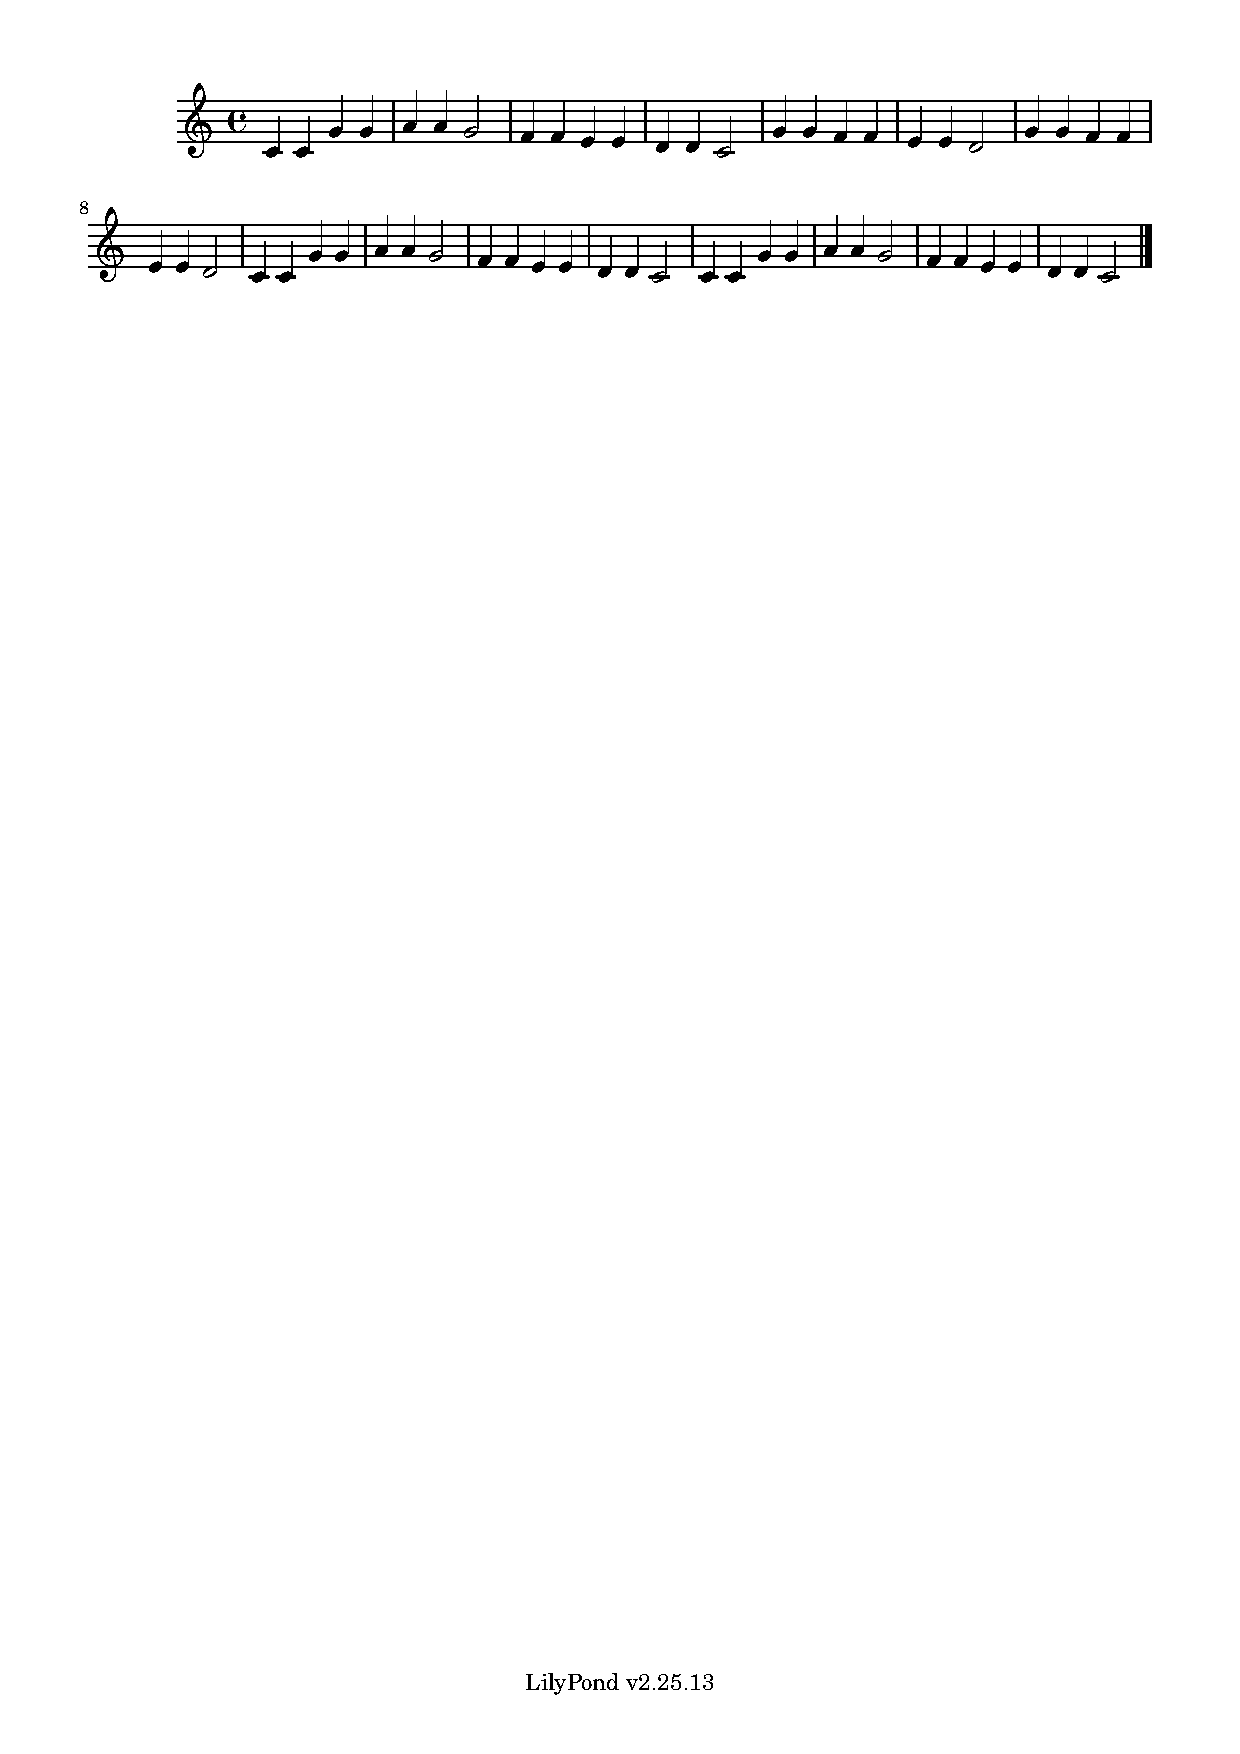
\includegraphics[trim=1cm 26.5cm 8.07cm 0.02cm, clip, scale=1]{dabby_1.pdf} % trim={left bottom right top}
\caption{The original of 12 variations on Ah vous dirai-je Maman in the first 4 bars.}
\label{fig:DabbyER1} 
\end{figure}

\begin{figure}
\centering
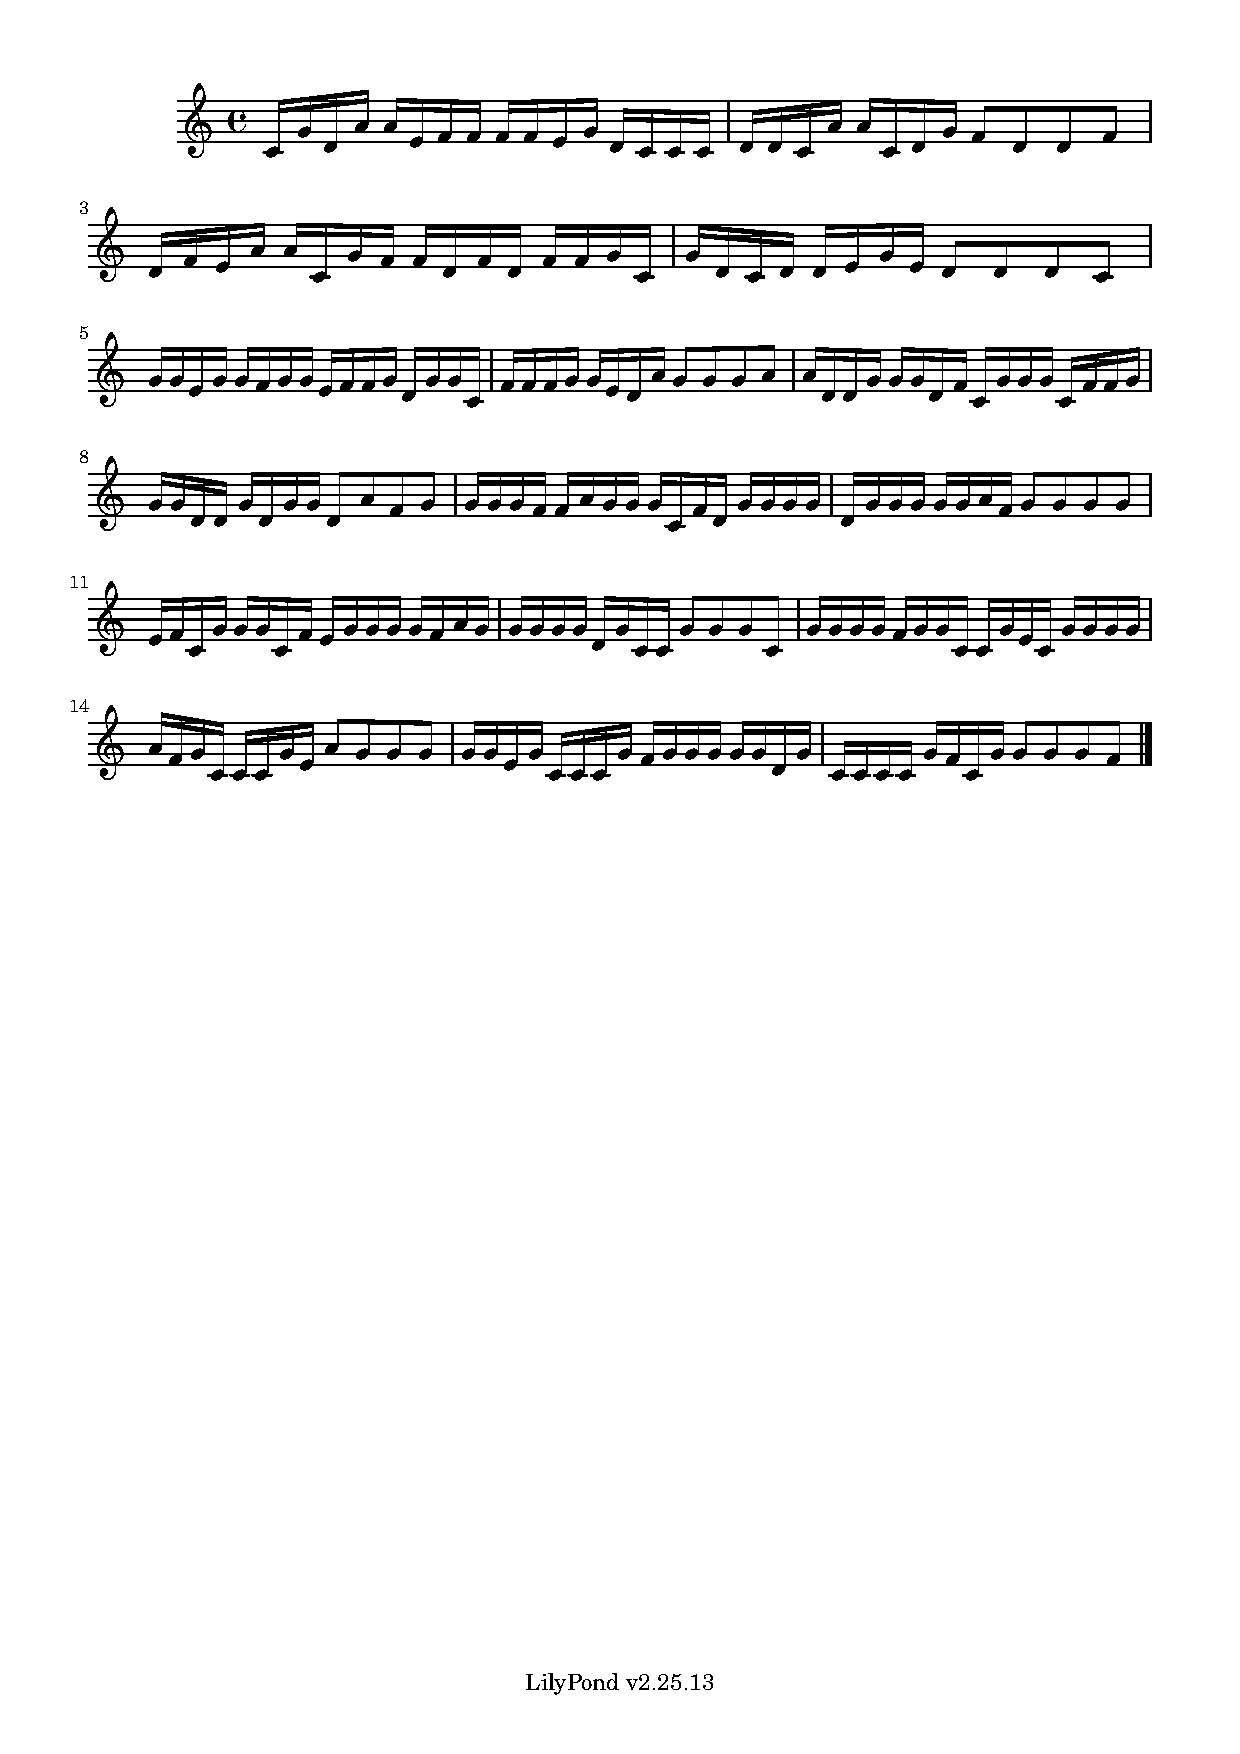
\includegraphics[trim=1cm 26.5cm 8.65cm 0.5cm, clip, scale=1]{dabby_melody_variation.pdf}
\caption{The new variation with melodic variation of Ah vous dirai-je, maman in the first bars, generated by the Initial Condition $(0.6, 0.5, 0.5)$.} 
\label{fig:DabbyER2}
\end{figure}

\begin{figure}
\centering

\begin{subfigure}{\textwidth}
  \centering
  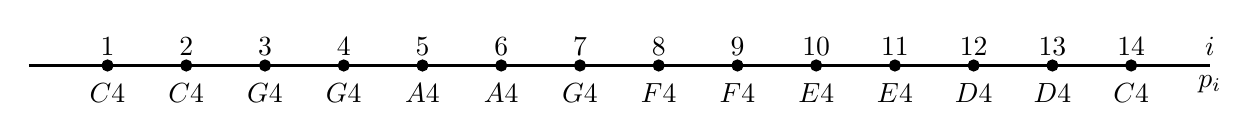
\begin{tikzpicture}
    % Draw number line
    \draw[-, thick] (0,0) -- (15,0) node[below] {$p_i$}  node[above] {$i$};

    % Data
    \foreach \i/\x/\p in {1/C4/1, 2/C4/2, 3/G4/3, 4/G4/4, 5/A4/5, 6/A4/6, 7/G4/7, 8/F4/8, 9/F4/9, 10/E4/10, 11/E4/11, 12/D4/12, 13/D4/13, 14/C4/14} {
      % Draw points and labels
      \filldraw (\i,0) circle (2pt) node[above] {$\p$};
      
      % Draw number scale below the line
      \draw (\i,-0.1) node[below] {$\x$};
    }

	\end{tikzpicture}
  \caption{The first 14 pitches of the 12 variations on Ah vous dirai-je Maman are marked below the pitch axis.}
  \label{subfig2:mp}
\end{subfigure}

\vspace{5pt}

\begin{subfigure}{\textwidth}
  \centering
  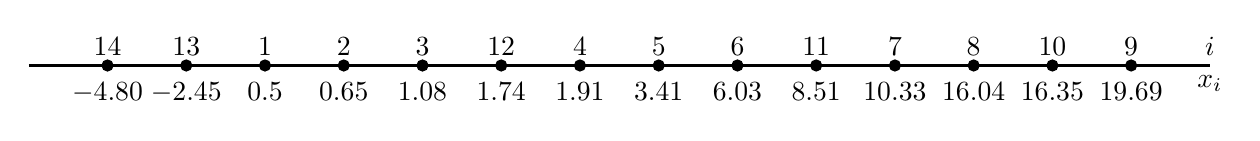
\begin{tikzpicture}
    % Draw number line
    \draw[-, thick] (0,0) -- (15,0) node[below] {$x_{i}$}  node[above] {$i$};

    % Data
    \foreach \i/\x/\p in {1/-4.80/14, 2/-2.45/13, 3/0.5/1, 4/0.65/2, 5/1.08/3, 6/1.74/12, 7/1.91/4, 8/3.41/5, 9/6.03/6, 10/8.51/11, 11/10.33/7, 12/16.04/8, 13/16.35/10, 14/19.69/9} {
      % Draw points and labels
      \filldraw (\i,0) circle (2pt) node[above] {$\p$};
      
      % Draw number scale below the line
      \draw (\i,-0.1) node[below] {$\x$};
    }

  \end{tikzpicture}
  \caption{The first 14 x-components of the numerical solution of Lorenz system with initial condition of $(0.5,0.5,0.5)$ are marked below the x axis.}
  \label{subfig2:traj1}
\end{subfigure}

\vspace{5pt}

\begin{subfigure}{\textwidth}
  \centering
  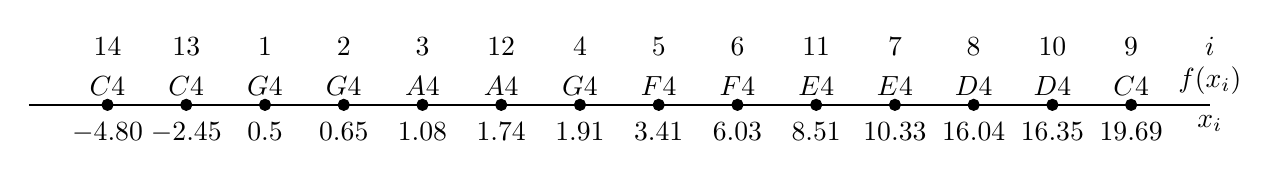
\begin{tikzpicture}
    % Draw number line
    \draw[-, thick] (0,0) -- (15,0) node[below] {$x_{i}$}  node[above] {$f(x_i)$} node[above=0.5cm] {$i$};

    % Data
    \foreach \i/\x/\p in {1/-4.80/C4, 2/-2.45/C4, 3/0.5/G4, 4/0.65/G4, 5/1.08/A4, 6/1.74/A4, 7/1.91/G4, 8/3.41/F4, 9/6.03/F4, 10/8.51/E4, 11/10.33/E4, 12/16.04/D4, 13/16.35/D4, 14/19.69/C4} {
      % Draw points and labels
      \filldraw (\i,0) circle (2pt) node[above] {$\p$};
      
      % Draw number scale below the line
      \draw (\i,-0.1) node[below] {$\x$};
    }
    
    % Display the sequence at each point
    \foreach \i/\x in {1/14, 2/13, 3/1, 4/2, 5/3, 6/12, 7/4, 8/5, 9/6, 10/11, 11/7, 12/8, 13/10, 14/9} {
      \draw (\i,0.5) node[above] {\x};
    }
  \end{tikzpicture}
  \caption{For each x-component $x_i$, apply the $f(x_{i})$ mapping.}
  \label{subfig2:traj1mp}

\end{subfigure}

\vspace{5pt}

\begin{subfigure}{\textwidth}
  \centering
  \small{
  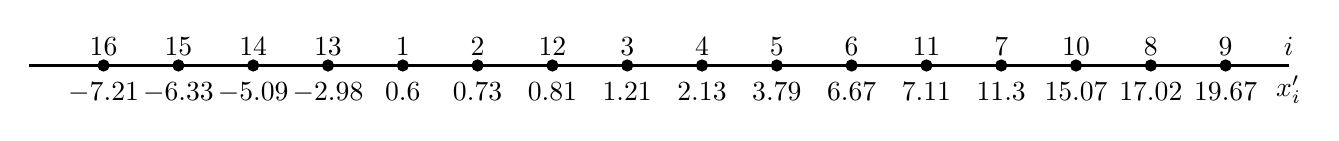
\begin{tikzpicture}
    % Draw number line
    \draw[-, thick] (0,0) -- (16,0) node[below] {$x^\prime_i$}  node[above] {$i$};

    % Data
    \foreach \i/\x/\p in {1/-7.21/16, 2/-6.33/15, 3/-5.09/14, 4/-2.98/13, 5/0.6/1, 6/0.73/2, 7/0.81/12, 8/1.21/3, 9/2.13/4, 10/3.79/5, 11/6.67/6, 12/7.11/11, 13/11.3/7, 14/15.07/10, 15/17.02/8, 16/19.67/9} {
      % Draw points and labels
      \filldraw (\i*0.95,0) circle (2pt) node[above] {$\p$};
      
      % Draw number scale below the line
      \draw (\i*0.95,-0.1) node[below] {$\x$};
    }

	\end{tikzpicture}}
  \caption{The first 16 x-components of the numerical solution of Lorenz system with new initial condition of $(0.6,0.5,0.5)$ are marked below the x axis.}
  \label{subfig2:traj2}

\end{subfigure}

\vspace{5pt}

\begin{subfigure}{\textwidth}
  \centering
  \small{
  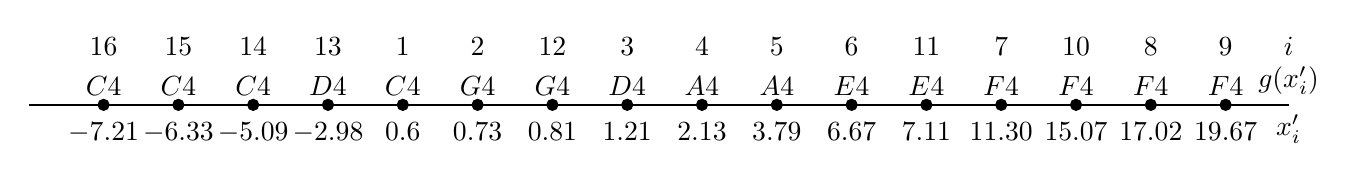
\begin{tikzpicture}
    % Draw number line
    \draw[-, thick] (0,0) -- (16,0) node[below] {$x^\prime_{i}$}  node[above] {$g(x^\prime_{i})$} node[above=0.5cm] {$i$};

    % Data
    \foreach \i/\x/\p in {1/-7.21/C4, 2/-6.33/C4, 3/-5.09/C4, 4/-2.98/D4, 5/0.6/C4, 6/0.73/G4, 7/0.81/G4, 8/1.21/D4, 9/2.13/A4, 10/3.79/A4, 11/6.67/E4, 12/7.11/E4, 13/11.30/F4, 14/15.07/F4, 15/17.02/F4, 16/19.67/F4} {
      % Draw points and labels
      \filldraw (\i*0.95,0) circle (2pt) node[above] {$\p$};
      
      % Draw number scale below the line
      \draw (\i*0.95,-0.1) node[below] {$\x$};
    }
    
    % Display the sequence at each point
    \foreach \i/\x in {1/16, 2/15, 3/14, 4/13, 5/1, 6/2, 7/12, 8/3, 9/4, 10/5, 11/6, 12/11, 13/7, 14/10, 15/8, 16/9} {
      \draw (\i*0.95,0.5) node[above] {\x};
    }
  \end{tikzpicture}}
  \caption{For each x-component $x^\prime_i$, apply the $g(x^\prime_{i})$ mapping.}
  \label{subfig2:traj2nmp}

\end{subfigure}

\vspace{5pt}

\begin{subfigure}{\textwidth}
  \centering
  \small{
  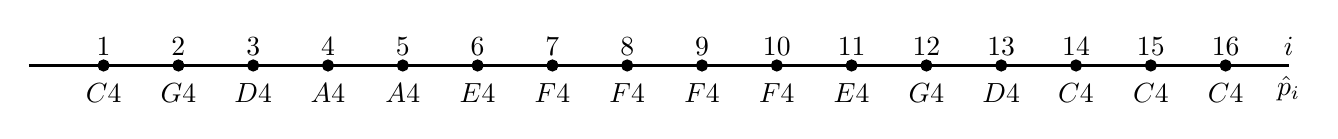
\begin{tikzpicture}
    % Draw number line
    \draw[-, thick] (0,0) -- (16,0) node[below] {$\hat{p}_i$}  node[above] {$i$};

    % Data
    \foreach \i/\x/\p in {1/C4/1, 2/G4/2, 3/D4/3, 4/A4/4, 5/A4/5, 6/E4/6, 7/F4/7, 8/F4/8, 9/F4/9, 10/F4/10, 11/E4/11, 12/G4/12, 13/D4/13, 14/C4/14, 15/C4/15, 16/C4/16} {
      % Draw points and labels
      \filldraw (\i*0.95,0) circle (2pt) node[above] {$\p$};
      
      % Draw number scale below the line
      \draw (\i*0.95,-0.1) node[below] {$\x$};
    }

	\end{tikzpicture}}
  \caption{The new variation of the first 11 pitches  are marked below the pitch axis.}
  \label{subfig2:nmp}

\end{subfigure}

\caption{The visualizes how a chaotic mapping with melodic variation method can be used to generate musical variations}
\label{fig2:dabbymv method}
\end{figure}

\end{document}